\documentclass{article}
\usepackage[top=30truemm,botom=30truemm,left=25truemm,right=25truemm]{geometry}
\usepackage{color}
\usepackage{amsmath}
\usepackage[dvipdfmx]{graphicx}
\begin{document}
VARIABLES
$t$: time

$x$: zonal position                                                        

$y$: meridional position                                                   

$\lambda$: longitude             

$\varphi$: latitude                                                      

$a$: the Earth radius                                                       

$p$: air pressure                                                        

$i$: grid number in x-direction                                            

$j$: grid number in y-direction                                            

$k$: grid number in vertival direction                                      

$q$: the amount of tracers *                                               

$u$: zonal velocity *                                                      

$v$: meridional velocity *                                                  

$F$: the flux of tracers ($uq$) *                                           

$G$: $uq\Delta y \Delta \sigma$ *                                           

$V$: $F$ when $q=1$ *

$\Delta D$: $\Delta D_{j,k}=a \cos \varphi_{j}\Delta \lambda \Delta \varphi_{j} \Delta \sigma$ *                               

$C$: the Courant number *                                             

$I_{C}$: integral fraction of the Courant number *                          

$\hat{C}$ decimal fraction of the Courant number *                         

$P^{S}$: Surface air pressure *                                         

$\sigma$: normalized pressure ($p/p^{S}$) *                               

$\eta$: $sigma$-$p$ hybrid coordinate *                              

$A$: the coefficient for $\eta$ coordinate *                               

$B$: the coefficient for $\eta$ coordinate *                       
                                                                           
  *: defined in this article    
\section{Tracer advection Scheme}
\subsection{Introduction of tracer advection scheme}
MIROC6 adopts spectral method based on Spherical harmonic expansion to dynamic core.
The spectral method is an excellent method, but it has some drawbacks.
\begin{enumerate}
\item Because of Gibbs phenomenon, noisy oscillations are produced when representing a field that is not smoot. 
\item Associated with Gibbs phenomenon, negative value may occure on grids whre they are not supposed to. ex.) specific humidity.
\item Global conservation of conservative quantity is good enough, but local conservation does not always hold.
\item The property that information is transmitted from upstream to downstream is not always satisfied. In spherical model, information travels instantly to the other side of the world.
\end{enumerate}
Despite of these disadvantages, MIROC has adoptted spectral method as dynamic core.
Gibbs phenomenon usually doesn't cause any problems. 
However, when describing the transport of materials with strong discontinuity, the noisy oscillation and unecpected negative values sometimes appear.
For example, water vapor in polar region and the stratosphere often shows discontinuous distribution because there is very small amount of water vapor.
Tracers such as aerosols are also distributed locally and often show large discontinuity.
These tracers are easy to affected by Gibbs phenomenon.
Therefore, in MIROC6, water vapor transport and tracer transport are calculated using flux form semi-Lagrange (FFSL) scheme (Lin and Rood 1996) instead of using the spectral method.

Merits of this scheme are described below.
\begin{enumerate}
\item Gibbs phenomenon doesn't occur because it's based on gridpoint method, it enables us to represent unsmooth fields with good accuracy. 
\item Negative values of tracer quantity can be avoided even in unsmooth fields.
\item No new extreme values are created.
\item Information is transmitted from upstream to downstream.
\item Conservation is satisfied locally and globally.
\item Problems which is induced by narrow grid range in polar region can be avoided.
\end{enumerate}
In the next section, the principle of the tracer advection scheme is introduced in detail, and in the follwing section, we describe the actual implementation of the tracer advection scheme.

\subsection{Principle of the tracer advection scheme}
\subsubsection{Transport equation in flux form}
The winds and the tracer distributions are staggered in the Arakawa C-grid (Mesinger and Arakawa 1976).
As example, three dimension advection equation in (x,y,p) rectangukar coordinate system is given as follows. 

\begin{equation}
\frac{\partial q}{\partial t} = -u \frac{\partial q}{\partial x}-v \frac{\partial q}{\partial y}-\omega \frac{\partial q}{\partial p}
\end{equation}
Here, $q$ is the amount of tracer (ex. specific humidity for water vapor), $u,v$ is zonal and merodinial velocity respectively.
By substituting continuity equation to this, we get the advection equation in flux form.
\begin{equation}
  \frac{\partial q}{\partial t}=-\frac{\partial}{\partial x}(uq)-\frac{\partial}{\partial y}(vq)-\frac{\partial}{\partial p}(\omega q)
  =-\frac{\partial}{\partial x}F^{x}-\frac{\partial}{\partial y}F^{y}-\frac{\partial}{\partial p}F^{p}
\end{equation}
Discretizing by $x=x_{i} (i=1,2,3...), y=y_{j} (j=1,2,3...), p=p_{k} (k=1,2,3...)$, the advection equation is rewritten as
\begin{equation}
  \frac{\partial q_{i,j,k}}{\partial t}=\frac{1}{\Delta x_{i,j,k}}(F^{x}_{i-\frac{1}{2},j,k}-F^{x}_{i+\frac{1}{2},j,k})+\frac{1}{\Delta y_{i,j,k}}(F^{y}_{i,j-\frac{1}{2},k}-F^{y}_{i,j+\frac{1}{2},k})+\frac{1}{\Delta p_{i,j,k}}(F^{p}_{i,j,k-\frac{1}{2}}-F^{p}_{i,j,k+\frac{1}{2}})
\end{equation}
Here, $F^{x}_{i-\frac{1}{2},j,k}$ is the flux in $x$ direction at boundary between $(i,j,k)$ and $(i-1,j,k)$, $\Delta x_{i,j,k}$ is x-direction width of grid represented as $(i,j,k)$.
This flux formed equation automatically satisfies conservation law. 
The accuracy of the scheme depends on how $F^{x}_{i-\frac{1}{2},j,k}$ is chosen.
Next, how $F^{x}_{i-\frac{1}{2},j,k}$ is determind in MIRIOC6 is explianed in one dimension in x-direction, for simplicity. 
\subsubsection{The Piecewise Parobolic Method (PPM) scheme}
In semi-Lagrange scheme, the flux of point $x_{i+\frac{1}{2}}$ at time $t$ is calculated by using $q$ of point $x_{i+\frac{1}{2}}-u\Delta t$ at time $t-\Delta t$.
The value of $u$ at time $t$, and $q$ at time $t-\Delta t$ are used.
If CFL condition ($|\frac{u\Delta t}{\Delta x}|<1$) is satisfied and $u_{i+\frac{1}{2}}>0$, $x_{i+\frac{1}{2}}-u\Delta t$ is at a point inside grid $i$.

As the value of $q$ at point $x_{i+\frac{1}{2}}-u\Delta t$, $q_{i}$, which is the average value of point $i$, can be chosen, assuming that $q$ is constant in the grid. 

However, the value of $q$ shows large discontinuity at $i+\frac{1}{2}$, which is the boundary between grid $i$ and $i+1$ in this assumption.
This discontinuity strengthens numerical viscosity, and is unwanted for numerical experiments. 
Therefore, we want to give some kind of distribution to $q$, which is assumed to be constant in a grid, in order to eliminate the discontinuity and enable us to calculate $q$ at $x_{i+\frac{1}{2}}-u\Delta t$ by interpolation.
Given distribution must be satisfied a condition as follows.
\begin{equation}
  q_{i}=\frac{1}{\Delta x_{i}} \int_{x_{i+\frac{1}{2}}}^{i-\frac{1}{2}} q(x) dx
\end{equation}

The old editions of MIROC adoptted van Leer method, in which interpolation function is a linear function, but MIROC6 adopts The Piecewise Parobolic Method (PPM) scheme (Colella and Woodward 1984) , in which interpolation function is a quadrative function (Fig.\ref{f1}). The FFSL scheme which adopts PPM scheme is called FFSL-3 (Lin and Rood 1996).

\begin{figure}
  \centering
  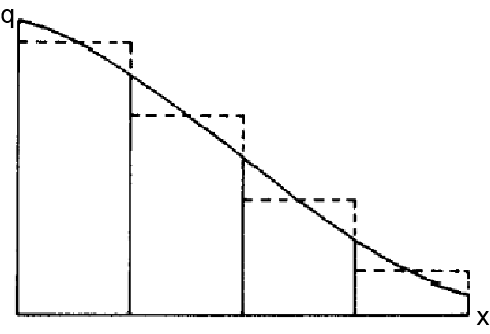
\includegraphics[width=5cm]{ppm_interpolate.png}
  \caption{The image of interpolation function in PPM scheme. The interpolation function is in the solid line, the grid mean value is in the dot line.}
  \label{f1}
\end{figure}

In PPM scheme, the distribution is determined as follows.
\begin{equation}
\begin{split}
\label{a4}
  q(x)=q_{L,i}+\xi (\Delta q_{i}+q_{6,i}(1-\xi))\\
  \xi=\frac{x-x_{i-\frac{1}{2}}}{\Delta x_{i}},  x_{i-\frac{1}{2}}\leq x \leq x_{i+\frac{1}{2}}
  \end{split}
\end{equation}
Here, $q_{L,i}$ is defined as $\lim_{x \to x_{i+\frac{1}{2}}}=q_{L,i}$.
$q_{R,i}$ is defined as $\lim_{x \to x_{i+\frac{1}{2}}}=q_{R,i}$ as well.
In PPM scheme, $q$ is continuous at boundary $i+\frac{1}{2}$, therefore $q_{L,i+1}=q_{R,i}=q_{i+\frac{1}{2}}$ is hold.
In addition, 
\begin{equation}
  \Delta q_{i}=q_{R,i}-q_{L,i},\qquad q_{6,i}=6(q_{i}-\frac{1}{2}(q_{L,i})+q_{R,i})
\end{equation}


For calculationg $q_{i+\frac{1}{2}}$ by interpolation, a finite integration of $q$ given as follows is introduced. 
\begin{equation}
  A(x)= \int^{x} q(x') dx'
\end{equation}
At boundary of grid,
\begin{equation}
A(x_{i+\frac{1}{2}})=A_{i+\frac{1}{2}}=\sum_{k\leq i}q_{k}\Delta x_{k}  
\end{equation}
$q_{i+\frac{1}{2}}$ is calculated by discretization of $q_{i+\frac{1}{2}}=dA/dx |_{x_{i+\frac{1}{2}}}$ by using $(A_{j+k+\frac{1}{2}},x_{j+k+\frac{1}{2}})$, $k=0,\pm 1, \pm 2$.
Specifically, $q_{i+\frac{1}{2}}$ is calculated as follows.
\begin{equation}
  \label{a3}
  \begin{split}
    q_{i+\frac{1}{2}}=&q_{i}+\Delta x_{i} \frac{q_{i+1}-q_{i}}{\Delta x_{i+1}+\Delta x_{i}}+\frac{1}{\sum_{k=i-1}^{i+2}\Delta x_{k}}\\
    &\times \Bigl[\frac{2\Delta x_{i}\Delta x_{i+1}}{\Delta x_{i+1}+\Delta x_{i}}(\frac{\Delta x_{i}+\Delta x_{i-1}}{\Delta x_{i+1}+2\Delta x_{i}}-\frac{\Delta x_{i+2}+\Delta x_{i+1}}{2\Delta x_{i+1}+\Delta x_{i}})(q_{i+1}-q_{i})\\
     & -\Delta x_{i}\frac{\Delta x_{i}+\Delta x_{i-1}}{\Delta x_{i+1}+2\Delta x_{i}} \delta q_{i+1}+\Delta x_{i+1} \frac{\Delta x_{i+2}+\Delta x_{i+1}}{2\Delta x_{i+1}+\Delta x_{i}} \delta q_{i}\Bigr]
  \end{split}
\end{equation}
In case the grid width is equal in all grids, Eq.(\ref{a3}) can be simply rewritten as
\begin{equation}
  q_{i+\frac{1}{2}}=\frac{1}{2}(q_{i-1}+q{i})-\frac{1}{6}(\delta q_{i}-\delta q_{i-1})
\end{equation}
Here, $\delta q_{i}$ is given as
\begin{equation}
  \delta q_{i}=\frac{\Delta x_{i}}{\Delta x_{i-1}+\Delta x_{i}+\Delta x_{i+1}}\biggl[\frac{2\Delta x_{i-1}+\Delta x_{i}}{\Delta x_{i+1}+\Delta x_{i}}(q_{i+1}-q_{i})+\frac{\Delta x_{i}+2\Delta x_{i+1}}{\Delta x_{i-1}+\Delta x_{i}}(q_{i}-q_{i-1})\biggr]
\end{equation}

However, in this case, the interpolation function may have extremes in the grid and may not satisfy monotonicity.
In order to avoid such a situation, $q_{i+\frac{1}{2}}$ should be between $q_{i}$ as $q_{i+1}$, and $\delta q_{i}$ is modified as follows for that. 
\begin{equation}
  \begin{aligned}
    \delta_{m} q_{i} & =\min(|\delta
    q_{i}|,2|q_{i}-q_{i-1}|,|q_{i+1}-q_{i}|) && \qquad \text{if$\quad(q_{i+1}-q_{i})(q_{i}-q_{i-1}) >0$}, \\
    & =0 && \qquad \text{otherwise}
  \end{aligned}
\end{equation}
This $\delta q_{i}$ is used in Eq.(\ref{a3}) to calculate $q_{i+\frac{1}{2}}$.

When $q(x)$ is interpolated as Eq.(\ref{a4}), by using Courant number defined as
\begin{equation}
  C=\frac{u_{i+\frac{1}{2}}\Delta t}{\Delta x_{i+1}}
\end{equation}
flux $F^{x}_{i+\frac{1}{2}}$ is wriiten as follows.
\begin{equation}
  F^{x}_{i+\frac{1}{2}}=\begin{cases}u_{i+\frac{1}{2}}[q_{R,i}-\frac{C}{2}(\Delta q_{i}-(1-\frac{2}{3}C)q_{6,i})] & (u_{i+\frac{1}{2}}\ge0)\\
  u_{i+\frac{1}{2}}[q_{L,i+1}+\frac{C}{2}(\Delta q_{i+1}+(1-\frac{2}{3}C)q_{6,i+1})] & (u_{i+\frac{1}{2}}\leq0)
  \end{cases}
\end{equation}
\subsubsection{Devices for taking long time steps}
The above argument is stable only if $C<1$
When the grid method is adapted to spherical coordinate, $\Delta x$ is very small in polar region.
Therefore, we have to take very small $\Delta t$ to satisfy CFL condition. 
The method for avoiding $C>1$ and taking larger $\Delta t$ are described below.
Although this method is used for any grid widths, in this subsection we assume that $\Delta x$ does not depend on $i$ for simplicity. 

Courant number can be divided into a integral fraction and a decimal fraction. 
\begin{equation}
  C=I_{C}+\hat{C},\quad I_{C}: a integral fraction,\quad -0.5\le \hat{C} \le 0.5
\end{equation}
When $I_{C}>0$
\begin{equation}
  F^{x}_{i-\frac{1}{2}}=\hat{F^{x}_{i-I_{C}+\frac{1}{2}}}+\sum^{i}_{i'=i+1-I_{C}} q_{i'} \frac{\Delta x_{i}}{\Delta t}
\end{equation}
When $I_{C}<0$
\begin{equation}
  F^{x}_{i-\frac{1}{2}}=\hat{F^{x}_{i+|I_{C}|+\frac{1}{2}}}+\sum^{i+|I_{C}|}_{i'=i+1} q_{i'} \frac{\Delta x_{i}}{\Delta t}
\end{equation}
Where $\hat{F^{x}_{i-I_{C}+\frac{1}{2}}}$ is the flux of point $(i-I_{C}+\frac{1}{2})$ calculated by using $\hat{C}$.

As indicated above, in the case the fluid moves in multiple grids during $\Delta t$, we can avoid instability of numerical calculation by evaluating the flux using the quantity $q_{i'}$ corresponding to each grids passed.
In actual, these argument is applied only to zonal flux, which can break CFL condition.

\subsubsection{The treatment of cross terms}
In the case velocity of the fluid is not only in the x-direction or y-direction, only adding the flux contributions in the x- and y-directions together underestimate the effect of diagonal advection. 
To take these cross term into considering, the following procedure is taken.
Here, we discuss this in two-dimensional space, not in one-dimensional.

When calculating x-direction flux $F^{x}_{i+\frac{1}{2},j}$, upstream value of $q$ in y-direction is used as value of $q$.
That is expressed by the following equation.
  \begin{equation}
    q^{y}_{i,j}=\frac{1}{2} {q(x_{i},y_{i}-v_{i,j}\Delta t)+q_{i,j}}
  \end{equation}
Here, $q(x_{i},y_{i}-v_{i,j}\Delta t)$ is calculated by linear interpolation of the two nearest grid points.
In the same way, when calculating y-direction flux $F^{x}_{i+\frac{1}{2},j}$,
  \begin{equation}
    q^{x}_{i,j}=\frac{1}{2} {q(x_{i}-u_{i,j}\Delta t,y_{i})+q_{i,j}}
  \end{equation}
  is used as $q$.

  In the case of three dimensional tracer advection, this procedure is conducted in two dimension.
  
  \subsection{Actual tracer advection scheme in MIROC6}
  In this subsection, actual procedure of the tracer advection scheme is described.
  Although MIROC6 adopts $\sigma -p$ hybrid coordinate as vertical coordinate, the tracer advection scheme is largely based on $\sigma$ coordinate because previous version of MIROC adopted $\sigma$ coordinate. 
  Therefore, firstly the procedure under $\sigma$ coordinate system is described.
  After this, the changes in the hybrid coordinate system from the $\sigma$ coordinate system is described.
  \subsubsection{$\sigma$ coordinate)}
The transport equation in $\sigma$ coordinate on the sphere is expressed as
\begin{eqnarray}
  \label{b1}
  \frac{\partial P^{S} q}{\partial t} &=& - \frac{1}{a \cos \varphi} \frac{\partial}{\partial \lambda}(P^{S} uq)- \frac{1}{a \cos \varphi} \frac{\partial}{\partial \varphi}(P^{S} vq \cos \varphi)- \frac{\partial}{\partial \sigma} (P^{S} \dot{\sigma} q)\\
  &=& \frac{1}{a \cos \varphi} \frac{\partial}{\partial \lambda}(F^{\lambda})- \frac{1}{a \cos \varphi} \frac{\partial}{\partial \varphi}(F^{\varphi})- \frac{\partial}{\partial \sigma} (F^{\sigma})
\end{eqnarray}
$P^{S}$ is surface pressure, $q$ is quantity of tracers.
Continuity equation is given by considering the case of $q=1$.
\begin{equation}
  \frac{\partial P^{S}}{\partial t} = - \frac{1}{a \cos \varphi} \frac{\partial}{\partial \lambda}(P^{S}u)- \frac{1}{a \cos \varphi} \frac{\partial}{\partial \varphi}(P^{S}v \cos \varphi)- \frac{\partial}{\partial \sigma} (P^{S} \dot{\sigma})
\end{equation}
Assuming that grid is equally spaced in zonal direction, the transport equation is discretized as follows.
\begin{equation}
\label{a1}
  \frac{\partial P^{S}_{,i,j,k} q_{i,j,k}}{\partial t}=\frac{1}{\Delta D_{j,k}}[(G^{\lambda}_{i-\frac{1}{2},j,k}-G^{\lambda}_{i+\frac{1}{2},j,k})+(G^{\varphi}_{i,j-\frac{1}{2},k}-G^{\varphi}_{i,j+\frac{1}{2},k}))+(G^{\sigma}_{i,j,k-\frac{1}{2}}-G^{\sigma}_{i,j,k+\frac{1}{2}})]
\end{equation}
Here,
\begin{equation}
  G^{\lambda}_{i-\frac{1}{2},j,k}=F^{\lambda}_{i-\frac{1}{2},j,k} \Delta y_{j} \Delta \sigma_{k}=(P^{S}uq)_{i-\frac{1}{2},j,k} \Delta y_{j} \Delta \sigma_{k}
\end{equation}
\begin{equation}
  G^{\varphi}_{i,j-\frac{1}{2},k}=F^{\varphi}_{i,j-\frac{1}{2},k} \Delta x_{j-\frac{1}{2}} \Delta \sigma_{k}=(P^{s}vq)_{i,j-\frac{1}{2},k} \Delta x_{j-\frac{1}{2}} \Delta \sigma_{k}
\end{equation}
\begin{equation}
  G^{\sigma}_{i,j,k-\frac{1}{2}}=F^{\eta}_{i,j,k-\frac{1}{2}} \Delta x_{j} \Delta y_{j}=(P^{S} \dot{\sigma} q)_{i,j,k-\frac{1}{2}} \Delta x_{j} \Delta y_{j}
\end{equation}
And
\begin{equation}
  \Delta D_{j,k}=a \cos \varphi_{j} \Delta \lambda \Delta \varphi_{j} \Delta \sigma_{k},\quad \Delta x_{j}=a \cos \varphi_{j} \Delta \lambda,\quad \Delta y_{j}=a \Delta \varphi_{j}
\end{equation}
This flux form equation ensure the conservation.

For the calculation of the time-averaged mass flux across the cell boundary, the winds and the tracer distributions are staggered in the Arakawa C-grid (Mesinger and Arakawa 1976). Tne horizontal winds at the cell boundary, $u_{i-\frac{1}{2},j,k}, v_{i-\frac{1}{2},j,k}$, are reconstructed by using the mass convergence field in the spectral model and the discretized continuity eqution: 
\begin{equation}
  \frac{\partial P^{S}_{i,j,k} }{\partial t}=\frac{1}{\Delta D_{j,k}}[(V^{\lambda}_{i-\frac{1}{2},j,k}-V^{\lambda}_{i+\frac{1}{2},j,k})+(V^{\varphi}_{i,j-\frac{1}{2},k}-V^{\varphi}_{i,j+\frac{1}{2},k}))+(V^{\sigma}_{i,j,k-\frac{1}{2}}-V^{\sigma}_{i,j,k+\frac{1}{2}})]
\end{equation}
Here, $V^{\lambda}_{i-\frac{1}{2},j,k}, V^{\varphi}_{i,j-\frac{1}{2},k}, V^{\sigma}_{i,j,k-\frac{1}{2}}$ denote zonal, meridional, and vertical mass-weighted wind at the cell boundary, rspectively. That is, 
\begin{equation}
  V^{\lambda}_{i-\frac{1}{2},j,k}=(P^{S}u)_{i-\frac{1}{2},j,k} \Delta y_{j} \Delta \sigma_{k}
\end{equation}
\begin{equation}
  V^{\varphi}_{i,j-\frac{1}{2},k}=(P^{S}v)_{i,j-\frac{1}{2},k} \Delta x_{j-\frac{1}{2}} \Delta \eta_{k}
\end{equation}
\begin{equation}
  V^{\sigma}_{i,j,k-\frac{1}{2}}=(P^{S}\dot{\sigma})_{i,j,k-\frac{1}{2}} \Delta x_{j} \Delta y_{j}
\end{equation}
$\Delta D_{j,k}$ denotes the cell volume, and $\Delta x_{j}, \Delta y_{j}$, and $\Delta \sigma_{k}$ denote zonal, meridional and vertical width of the cell, respectively. That is $\Delta D_{j,k}=a \cos \varphi_{j}\Delta \lambda \Delta \varphi_{j} \Delta \sigma$, $\Delta x_{j}=a \cos \varphi_{j} \Delta \lambda$ and $\Delta y_{j}=a \Delta \varphi_{j}$.

The following are the procedure for the calculation of tracer advection in the staggering-grided horizontal and vertical wind fields:
\begin{enumerate}
\item Surface pressure $P^{S}(t+\Delta t)$ and horizontal wind $\bf{v}(t+\Delta t)$ are predicted in the spectral model.
\item The horizontal component of mass flux divergence at time step $t$ is calculated by using spherical harmonics. The mass fluxes at time step $t$ are reconstructed from the values at $t+\Delta t$ and $t-\Delta t$ because MIROC applies semi-implicit scheme for the time-integration of surface pressure. Zonal and meridional component of mass flux divergence are: 
  \begin{equation}
    C^{x}=-\frac{1}{a \cos \varphi}\frac{\partial}{\partial \lambda}(P^{s}u),\quad C^{y}=-\frac{1}{a \cos \varphi}\frac{\partial}{\partial \lambda}(P^{s}v \cos \varphi) 
  \end{equation}
\item By using $C_{x}$ and $C_{y}$, $V^{\lambda}, V^{\varphi}, V^{\sigma}$ are calculated as follows.
  \begin{equation}
    V^{\lambda}_{i-\frac{1}{2},j,k}-V^{\lambda}_{i+\frac{1}{2},j,k}=C^{x}_{i,j,k}\Delta D_{j,k}, \quad V^{\lambda}_{i,j-\frac{1}{2},k}-V^{\lambda}_{i,j+\frac{1}{2},k}=C^{y}_{i,j,k}\Delta D_{j,k}
  \end{equation}
  The boundry conditions are $V^{\varphi}=0$ at the North Pole and South Pole、$\sigma=1$ at surface and $V^{\sigma}=0$ at $\sigma=0$.
The condition for $V^{\lambda}=0$ is:
  \begin{equation}
    \sum_{i}V^{\lambda}_{i-\frac{1}{2},j,k}=\sum_{i}P^{S}_{i,j,k}u_{i,j,k}\Delta y_{j}\Delta \sigma_{k}
  \end{equation}
  That means zonal mean of zonal mass transport is equal to that in the spectral model grid.
  Here, the following equation must be satisfied for boundary condition $V^{\varphi}=0$ at the North Pole and the South Pole. 
  \begin{equation}
    \sum_{j}C^{y}_{i,j,k}\Delta D_{j,k}=0
  \end{equation}
  However, this is not always satisfied (On the other hand, $\sum_{i} \sum_{j}C^{y}_{i,j,k}\Delta D_{j,k}=0$ is valid within numerical error.).

  In order to satisfy the boundary condition, the following correction is made.
  \begin{equation}
    C^{y}_{i,j,k}\leftarrow C^{y}_{i,j,k}-\delta C, \quad C^{y}_{i,j,k}\leftarrow C^{x}_{i,j,k}+\delta C
  \end{equation}
  Here, $\delta C=\sum_{j}C^{y}_{i,j,k}\Delta D_{j,k}/\sum_{j}\Delta D_{j,k}$.
  Vertical velocity $V^{\eta}$ is obtained by using
  \begin{equation}
    \label{a2}
    \frac{\partial P^{S}_{i,j,k}}{\partial t}\sum_{k}\Delta D_{j,k}=\sum_{k}(C^{x}_{i,j,k}+C^{y}_{i,j,k})
  \end{equation}
  (The contents so far are in [TRACEG]。The rest of the content is in [GTRACE])
\item $G^{\lambda}, G^{\varphi}, G^{\sigma}$ are calculated by PPM scheme from $V^{\lambda}, V^{\varphi}, V^{\sigma}$.

\item $P^{s}_{i,j,k}q_{i,j,k}$ at time step $t+\Delta t$ is calulated by integration of Eq.(\ref{a1}) by leap frog method from $G^{\lambda}, G^{\varphi}, G^{\sigma}$.

\item $q_{t+\Delta t}$ is calculated by dividing $(P^{s}q)_{t+\Delta t}$ by $P^{s}_{t+\Delta t}$.
  There is small quantity of difference between $P^{s}_{t+\Delta t}$ from Eq. (\ref{a2}) and $P^{s}_{t+\Delta t}$ in the spectral model, because semi-implicit time integration scheme is applied.
  $P^{s}_{t+\Delta t}$ from Eq. (\ref{a2}) is applied at present for the consistency of mass advection. Mass Conservation is not strictly satisfied because of the discrepancy between the surface pressure in the spectral model and from $P^{s}_{t+\Delta t}$ Eq. (\ref{a2}).
\end{enumerate}

\subsubsection{$\sigma-p$ hybrid coordinate}
The transport equation in $\eta$ coordinate ($\sigma-p$ hybrid coordinate) on the sphere is: 
\begin{eqnarray}                                                             \frac{\partial mq}{\partial t} &=& - \frac{1}{a \cos \varphi} \frac{\partial}{\partial \lambda}(muq)- \frac{1}{a \cos \varphi} \frac{\partial}{\partial \varphi}(mvq \cos \varphi)- \frac{\partial}{\partial \eta} (m \dot{\eta} q)\\                                                                         &=& \frac{1}{a \cos \varphi} \frac{\partial}{\partial \lambda}(F^{\lambda})- \frac{1}{a \cos \varphi} \frac{\partial}{\partial \varphi}(F^{\varphi})-\frac{\partial}{\partial \eta} (F^{\eta})                                    
\end{eqnarray}
Here,$m$ corresponds to the density of the coordinate and is defined as $m=\frac{\partial p}{\partial \eta}$.
if you look at Eq. (\ref{b1}), you can find that difference of $\sigma$ coordinate and $\eta$ coordinate is only that $P^{S}$ replaces $m$.
The actual tracer advection in $\eta$ coordinate is mostly the same as $\sigma$ coordinate.  

In the scheme in $\eta$ coordinate, the following variables are calculated in the same way as the way $G^{\lambda}, G^{\varphi}, G^{\eta}$ is calculated in $\sigma$ coordinate, except $\Delta \sigma$ replaces with $\Delta \eta$ and $\dot{\sigma}$ replaces with $\dot{\eta}$. 
\begin{equation}
  G^{\prime \lambda}_{i-\frac{1}{2},j,k}=(P^{S}uq)_{i-\frac{1}{2},j,k} \Delta y_{j} \Delta \eta_{k},\quad G^{\prime \varphi}_{i,j-\frac{1}{2},k}=(P^{S}vq)_{i,j-\frac{1}{2},k} \Delta x_{j-\frac{1}{2}} \Delta \eta_{k},\quad G^{\prime \eta}_{i,j,k-\frac{1}{2}}=(P^{S} \dot{\eta} q)_{i,j,k-\frac{1}{2}} \Delta x_{j} \Delta y_{j}
\end{equation}
In the time integration step, multiplying $G\prime$ by $m/P^{S}$, $G^{\lambda}, G^{\varphi}, G^{\eta}$ is calculated.
After that, $mq$ at time step $t+\Delta t$ is calculated by leap-frog method as well as $\sigma$ coordinate.

In actual source code, conbining to dividing by $m$ to calculate $q$ at time step $t+\Delta t$, $q$ at point $(i,j,k)$ in time step $t+\Delta t$ is calculated as follows. 
\begin{equation}
  \begin{split}
        q^{t+\Delta t}=&\frac{\Delta A_{k}+\Delta B_{k} P^{S,t-\Delta t}_{i,j,k}}{\Delta A_{k}+\Delta B_{k} P^{S,t+\Delta t}_{i,j,k}}q^{t-\Delta t}_{i,j,k}+\frac{2\Delta t}{\Delta D}\\
    &\times [(G^{\prime \lambda,t}_{i-\frac{1}{2},j,k}-G^{\prime \lambda,t}_{i+\frac{1}{2},j,k})+(G^{\prime \varphi,t}_{i,j-\frac{1}{2},k}-G^{\prime \varphi,t}_{i,j+\frac{1}{2},k}))+(G^{\prime \eta,t}_{i,j,k-\frac{1}{2}}-G^{\prime \eta,t}_{i,j,k+\frac{1}{2}})]\\
    &\times \frac{\Delta A_{k}+\Delta B_{k} P^{S,t}_{i,j,k}}{P^{S,t}_{i,j,k}}\frac{1}{\Delta A_{k}+\Delta B_{k} P^{S,t+\Delta t}_{i,j,k}}
  \end{split}
\end{equation}
Here,$A,B$ is the coefficients for $\eta$ coordinate, $\eta_{k+\frac{1}{2}}=A_{k+\frac{1}{2}}/p_{0}+B_{k+\frac{1}{2}}$ and $\Delta A_{k}=A_{k-\frac{1}{2}}-A_{k+\frac{1}{2}},\quad \Delta B_{k}=B_{k-\frac{1}{2}}-B_{k+\frac{1}{2}}$.
And $\Delta A_{k}+\Delta B_{k} P^{S}_{i,j,k}=\Delta p_{i,j,k}$(More details in the section of the vertical discretization).

\subsubsection{The mass fluxes into/out of polar caps}
The mass fluxes into/out of polar caps are calculated by using the semi–Lagrangian scheme in the polar stereo projection (cf. Fig.\ref{f2}).
The horizontal average at the highest latitude band is assumed to be preserved before/after flux calculation for the mass conservation. The sequence of calculation is:
\begin{enumerate}
\item Zonal average of $P^{S}q$ at time step $t$ is calculated at the highest latitude band $(j=j_{N},j_{S})$, and is assumed to equal $P^{S}q$ at the pole.
\item Horizontal wind at the highest latitude bands is projected into the orthogonal coordinate system centering around the pole, and $q$ at time step $t + \Delta t$ is estimated by using the value at the “departure point”.
\item Zonal anerage of $P^{S}q$ at time step $t+\Delta t$ is fixed to that at $t$.
\end{enumerate}

\begin{figure}
  \centering
  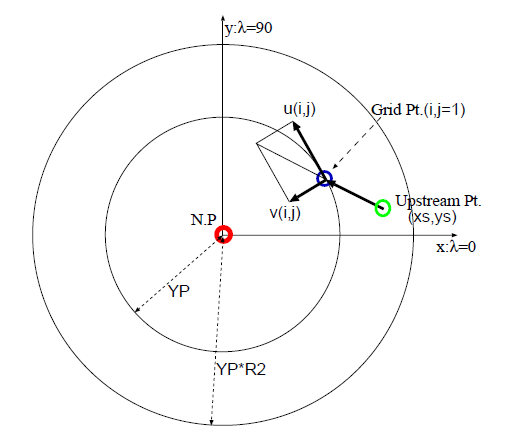
\includegraphics[width=5cm]{polar_tracer_advection.png}
  \caption{Conceptual figure for the flux on pole-most grids.}
  \label{f2}
\end{figure}
\end{document}
